\chapter{Gamification}
\label{gamification}

Unter \gls{Gamification} versteht man die Verwendung von spieltypischen Elementen in einem spielfremden Kontext.
Die bekanntesten Elemente dabei sind die Punktevergabe für das Lösen von Aufgaben, die Verleihung von Badges für besonders engagierte Einsätze oder das Bereitstellen einer Highscore zum Vergleich mit anderen Benutzern.

Während unserer Arbeit hatten wir verschiedene Partner, welche uns bei der \gls{Gamification} unserer Applikation unterstützen.
So ist einer unserer Industriepartner Mitinhaber der Firma bitforge AG\footnote{\url{http://bitforge.ch/}}, welche sich auf Games im mobilen Umfeld spezialisiert hat.
Er konnte uns vor und während der Entwicklung viele wertvolle Tipps zur Verbesserung des Spielgefühls geben.

\section{Gamification in Kort}
\subsection{Sprache}
\gls{Gamification} findet sich nicht nur in schönen Grafiken und Spiel-Elementen.
Sie beginnt bereits bei der Sprachwahl von Texten.
Beim Lesen der Texte sollte beispielsweise eine gewisse Spannung aufgebaut werden.
Dadurch erhöht sich die Motivation die anstehende Aktion durchzuführen.

In \kort{} findet sich dafür ein Beispiel in der Button-Bezeichnung bei der Eingabe des eigenen Benutzernamens.
Zu Beginn war dieser mit "`App starten"' beschriftet.
Wir haben ihn aber später mit dem Text "`Mission beginnen!"' ersetzt.
Weiter wurde der Button grün eingefärbt, um ihn zusätzlich vom Text und vom Hintergrund abzuheben.

\begin{figure}[H]
	\centering
	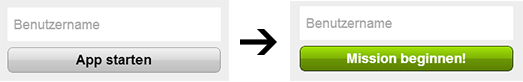
\includegraphics{images/gamification/gamification-lang-firststeps}
	\caption{Gamification - Sprache}
	\label{gamification-lang-firststeps}
\end{figure}

Neben der gewählten Ausdrucksweise sollte die Sprache dem Zielpublikum angepasst werden.
Wir mussten dafür viele Begriffe aus dem \glslink{Mapper}{Mapping}-Vokabular für unserer breite Zielgruppe mit allgemeineren Wörtern ersetzen.

\subsection{Punktesystem "`Koins"'}
Eines der wichtigsten Elemente im Spiel bildet das Punktesystem. Dieses findet sich in beinahe allen Aktionen der App wieder.
So gewinnt ein Spieler für gelöste Aufgaben oder getätigte Prüfungen eine gewisse Anzahl an sogenannten \emph{Koins}.
Über die Anzahl \emph{Koins} kann er sich wiederum in der Highscore mit den anderen Spieler messen.

\begin{figure}[H]
	\centering
	
\includegraphics[scale=0.4]{images/gamification/gamification-koin}
	\caption{Gamification - Koins}
	\label{gamification-koins}
\end{figure}

\subsection{Auszeichnungen}
Zusätzlich zu den \emph{Koins} kann ein Spieler Auszeichnungen gewinnen. Diese erhält man durch besondere Leistungen. In \kort{} sind momentan folgende Auszeichnungen implementiert:

\begin{table}[H]
\centering
\begin{tabular}{|p{0.25\twocelltabwidth}|p{0.75\twocelltabwidth}|}
\hline 
\textbf{Auszeichnungstyp} & \textbf{Beschreibung} \\ 
\hline 
Anfänger & Eine Auszeichnungen für das Lösen des 1. Auftrags und eine für das Überprüfen der 1. Antwort. \\ 
\hline 
Platzierung & Drei Auszeichnungen für das Erreichen des 1., 2. und 3. Rangs in der Highscore. \\ 
\hline 
Aufträge & Drei Auszeichnungen für das Lösen von 10, 50 und 100 Auträgen. \\ 
\hline 
Prüfungen & Drei Auszeichnungen für 10, 10 und 1000 geprüfte Antworten. \\ 
\hline 
\end{tabular} 
\caption{Auszeichnungen in Kort}
\label{kort-badges}
\end{table}

\begin{figure}[H]
	\centering
	
\includegraphics[scale=0.7]{images/gamification/gamification-badges}
	\caption{Gamification - Badges}
	\label{gamification-badges}
\end{figure}

Das Hinzufügen von zusätzlichen Auszeichnungen wird in Abschnitt \ref{kort-additional-badges} beschrieben.

\subsection{Highscore}
Über die Highscore haben die Benutzer der App die Möglichkeit sich mit den anderen Spielern zu vergleichen.
Dazu werden sie nach Anzahl gewonnener \emph{Koins} in einer Rangliste eingestuft.

\section{Weitere mögliche Elemente}
Neben den verwendeten \gls{Gamification}-Elementen in \kort{} gibt es noch eine Vielzahl weiterer Elemente, welche sich für diesen Anwendungszweck eigenen würden.
Diese konnten während der Arbeit aber nicht implementiert werden.

Daneben gibt es aber auch noch Elemente welche zwar für \brand{OpenStreetMap} als Projekt interessant wären, sich jedoch nicht mit \kort{} umsetzen lassen.

\subsection{Erste Schritte}
Um den Einstieg in die Verwendung der App weiter zu vereinfachen wäre es sinnvoll beim ersten Start eine kurze Einführung anzuzeigen.
So könnte man dem Benutzer für die einzelnen Masken jeweils Tipps einblenden oder gar eine geführte Tour durch die App und deren Möglichkeiten anbieten.

Wenn der Benutzer nicht weiss, welche Möglichkeiten er hat, kann dies dazu führen, dass er schnell wieder aufgibt oder nicht das volle Potential der App ausschöpfen kann.

\subsection{Zeitlich begrenze Aktionen}
Durch das Einführen von zeitlich begrenzten Aktionen kann man Benutzer dazu motivieren die App über einen längeren Zeitraum zu verwenden.
So könnte man Tage definieren, an denen man die doppelte Anzahl an Punkten gewinnt.
Zusätzlich könnte man Aktionen\footnote{Beispiel einer zeitlich begrenzen Aktion in \brand{OpenStreetMap}: Das \brand{big baseball project 2011} \url{http://wiki.openstreetmap.org/wiki/Big_baseball_project_2011}} starten, bei denen man spezielle Auszeichnungen gewinnen kann.

Um den Benutzer dazu zu animieren die App erneut zu starten, könnte man per Push-Meldungen auf aktuelle Aktionen, Updates oder Ereignisse aufmerksam machen.

\subsection{Weitere Auszeichnungen hinzufügen}
Bei der Auswahl an verfügbaren Auszeichnungen sollte man darauf achten, dass es für jeden Spielertyp geeignete Auszeichnungen zu gewinnen gibt.
Die verschiedenen Typen haben eine ganz andere Herangehensweise und müssen deshalb auch mit verschiedenen Belohnungen motiviert werden.
Eine Einteilung von verschiedenen Spielertypen wird auf \brand{Gamasutra}\footnote{\url{http://www.gamasutra.com/view/feature/6474/personality_and_play_styles_a_.php}} beschrieben.

Es gibt bereits eine Liste von möglichen Badges im Wiki von OpenStreetMap\footnote{\url{https://wiki.openstreetmap.org/wiki/Badges}}.

\subsection{Verschiedene Highscores}
Durch das Bereitstellen von verschiedenen Highscores (Bsp. Regional, Nach Fehlertyp), gibt man allen Benutzern die Chance, irgendwo den ersten Platz zu erreichen.
Dadurch verhindert man eine mögliche Demotivation beim Vergleich mit Langzeitspielern, welche bereits eine grosse Anzahl an Punkten gesammelt haben.

\subsection{Erfahrene Spieler}
Man könnte als Belohnung für viele gelöste Fehler die Berechtigungen des Benutzers erhöhen.
So könnte beispielsweise seine Stimme bei einer Überprüfung einer Lösung doppelt zählen.
Dieses Prinzip wird auch von der Frage/Antwort-Plattform \brand{Stack Overflow}\footnote{\url{http://stackoverflow.com/}} angewendet.

\begin{figure}[H]
	\centering
	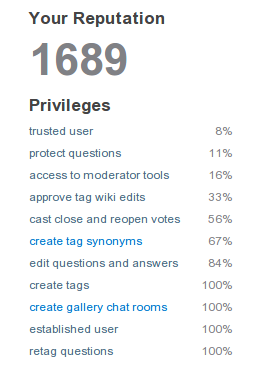
\includegraphics[scale=0.7]{images/gamification/so-privileges}
	\caption{Zusätzliche Berechtigungen bei StackOverflow}
	\label{gamification-so-privileges}
\end{figure}

Um erfahrene Spieler nicht zu unterfordern, könnte man ihm beim Erreichen einer gewissen Punktzahl, Fehler anzeigen, welche schwieriger zu lösen sind.
Wichtig ist es dabei, dass das Spiel nicht plötzlich vorbei ist.
Auch der Spieler der bereits die meisten Punkte hat, muss noch eine Motivation haben die App weiter zu verwenden.

\subsection{Einbinden in Apple Game Center}
Apple bietet mit dem \brand{Game Center} einen zentralen Ort an, Punkte und Auszeichnungen von Game-Apps zu speichern.
Dadurch entsteht für die Spieler die Möglichkeit sich direkt mit anderen Spielern und Kollegen, die ebenfalls diese App verwenden, zu vergleichen.
Dadurch, dass das \brand{Game Center} bereits eine grosse Community an Spielern aufweist, wäre es von Vorteil, die App darin einzubinden.
Leider besteht dabei die Einschränkung, dass man lediglich iOS-Games für das Game Center anmelden kann.

\subsection{Design}
Spiele habe viele Design-Eigenheiten, welche sich von reinen Business-Applikationen abheben.
Dies kann durch geeignete Farben und UI-Elemente realisiert werden.
Typischerweise wird ein Benutzer durch die Applikation geführt, so dass ihm immer klar ist wie es weiter geht.

\subsection{Gamification von OpenStreetMap}
In der \brand{OpenStreetMap} Community gibt es bereits einige Ideen um Spiele-Konzepte für das Projekt zu verwenden.
Beispielsweise gab es eine rege Diskussion auf der Geowanking-Mailingliste\footnote{\url{http://geowanking.org/pipermail/geowanking_geowanking.org/2012-September/thread.html\#26302}} welche durch Prof. Stefan Keller initiiert wurde.

An der State Of The Map Konferenz 2011 (SotM 2011) hat Martijn van Exel  einen Vortrag zum Thema \emph{Can gaming concepts help make OpenStreetMap better?}\footnote{\url{http://wiki.openstreetmap.org/wiki/SotM_2011_session:_Insert_Coin_To_Play}} gehalten.

Er beschreibt darin eines der Hauptprobleme von \brand{OpenStreetMap}, dass es neuen Benutzern schwerfällt die \emph{erste Meile} zurückzulegen.
Viele neue Benutzer haben Angst davor etwas falsch zu machen und müssen sich zuerst mit den vielfältigen Möglichkeiten des Karten-Editors vertraut machen.
Die Statistik der Benutzer von \brand{OpenStreetMap} bestätigt dieses Bild: fast Zweidrittel der Benutzer hat zwar ein Benutzerkonto, hat aber noch keine Änderungen vorgenommen.

Martijn van Exel schlägt deshalb vor, dass das Recht die Karte zu editieren gestaffelt werden soll.
So soll sich ein Benutzer das Recht "`verdienen"' müssen, komplexere Änderungen an der Karte vorzunehmen.

Dadurch kann der Spieltrieb des Menschen geweckt werden, um sich weiterzuentwickeln.
Nebenbei lernt der Benutzer den Umgang mit dem Karteneditor und fühlt sich sicherer überhaupt Änderungen vorzunehmen.